\documentclass[a4paper,11pt,oneside]{book}
\usepackage{style}
\usepackage{chapters/imf-language-overview/imf-language-visualisation/imf-style-tikz}
\usepackage{chapters/imf-language-overview/figure/ontology-diagram-style}
\usepackage{chapters/imf-language-overview/style}
\usepackage{subfiles}
\begin{document}
\setcounter{secnumdepth}{3}

\begin{titlepage}
  \centering
  {~ \par}
  \vspace{5.5cm}
  {\Huge\bfseries Information Modelling Framework Manual\par}
  \vspace{2cm}
  {\Large Version 0.3.0\par}
  \vfill        
  % Bottom of the page
  {\large \today\par}
\end{titlepage}


\frontmatter

\subfile{chapters/F-document-status}
%\subfile{chapters/F-document-description}
%\subfile{chapters/F-preface}
\subfile{chapters/F-outline}

\setcounter{tocdepth}{3}
\tableofcontents
%\listoffigures
%\listoftables
%\printglossary[title=List of Terms]
%\printglossary[type=\acronymtype, title=List of Acronyms]
%\glsaddallunused % include all defined terms and acronyms

\mainmatter

\subfile{chapters/M-scope}
\subfile{chapters/M-newway}
\subfile{chapters/M-fundamentals}
%\subfile{chapters/M-imfquickref}
%\subfile{chapters/M-imf-language-overview}
\subfile{chapters/imf-language-overview/subfile-main}
\subfile{chapters/M-howtomodel}
\subfile{chapters/M-howtotypes}


\printbibliography

%\appendix

%\subfile{chapters/A-contract}
%\subfile{chapters/M-imf-language}

%%%\chapter{Structural Specification}
\label{ch:Appendix C}
The structural specification is a format and application independent data model
specification of the formal specification of IMF. The structural specification aims to faithfully represent the
intentions of the formal specification while also including the specification of how, e.g., objects metadata and
attributes and attribute values are represented, which the formal specification does not contain. The purpose of the
structural specification is to be a common language and format for developing concrete serialization formats for IMF
and serve as documentation for application developers.

\begin{figure}[htb]
  \centering
  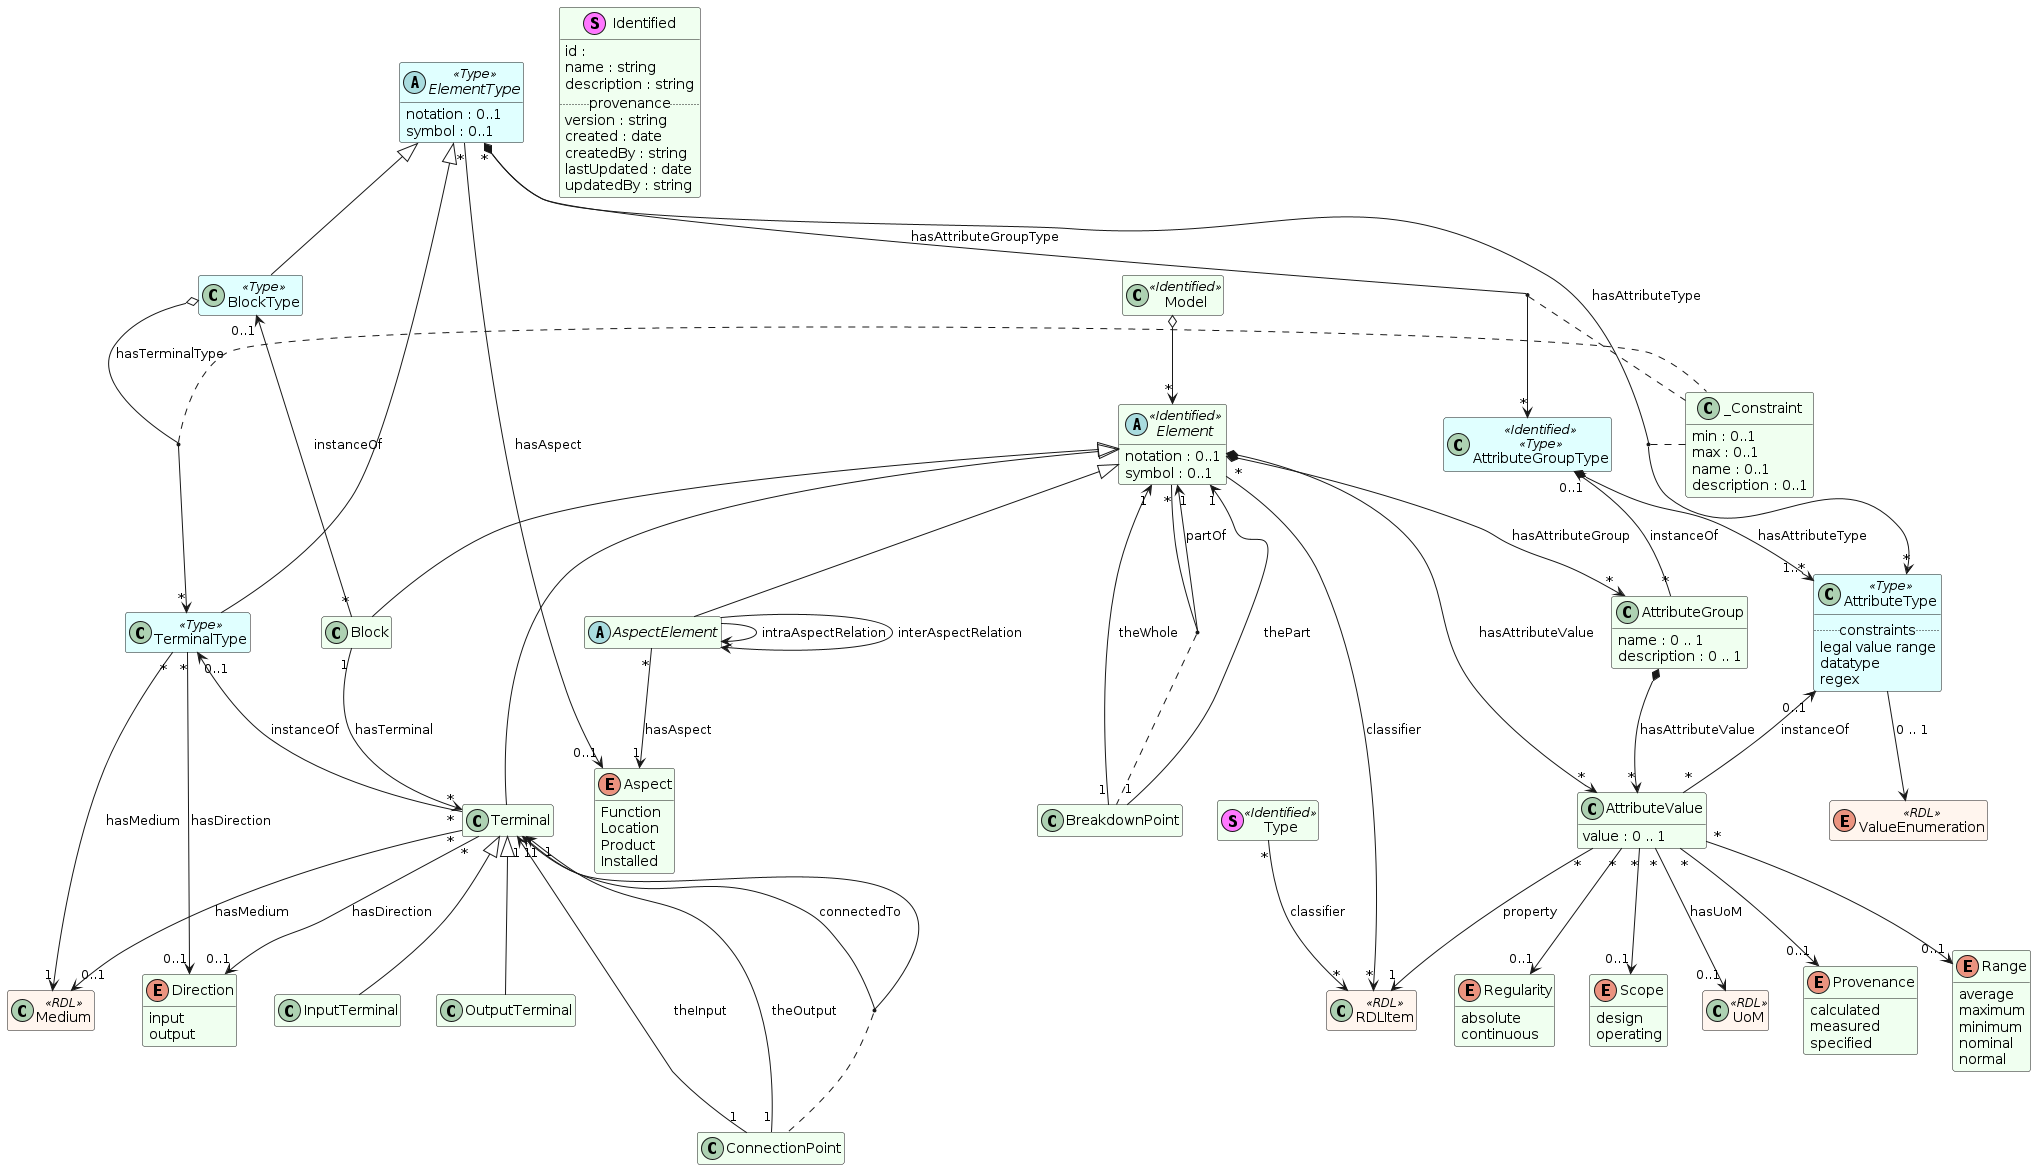
\includegraphics[width=1\textwidth]{img/IMFmanual-img073.png}
  \caption{The complete structural specification.}
  \label{fig:Figure 55}
\end{figure}
%%%\chapter{Semantic Verification
 }\label{ch:Appendix E}
IMF Types and Models are by design developed by reusing resources in an RDL. In order to
enable semantic verification, we assume that the RDL classes are provided in an OWL format that supports efficient
use of reasoning. ISO 15926-14 is an upper level ontology with exactly this ambition. We will in this chapter assume
that the classes and attributes referred to in IMF Types and IMF Blocks with Terminals lie in an RDL that implements ISO
15926-14.

The primary aim of semantic verification is to detect inconsistencies in an IMF Model. When this is achieved and
demonstrated, it is in the scope of IMF to support complex reasoning patterns based on inheritance of design
decisions, as well as encoding of engineering rules. An example of a potential inconsistency in an IMF Model, that
could be detected by a reasoning procedure, is conflicts between property restrictions in the definition of RDL
classes and the combination of RDL classes and attribute constraints in the definition of an IMF Types. There are
many ways in which the use of classes and attributes in IMF may clash with their definitions and position in an RDL
class hierarchy, and it is not likely that it is possible to inspect and check all these cases by manual methods when
an IMF model grows beyond a small toy example.

A natural step to this end would be to translate an IMF Model into an instance of an ISO 15926-14 ontology. There are
two reasons why this is not straightforward. First, IMF types are defined with constraints that cannot be expressed
in OWL. However, since validating an IMF Model with respect to such constraints can be achieved independently of
semantic verification, this is not an issue. We may just assume that the IMF Model has been validated with respect to
its constraints, e.g., by use of SHACL, prior to semantic verification and then we can safely ignore the constraints
in the semantic verification. Second, IMF Models are used to capture requirements and specifications, and it is not
clear how requirements and specifications can be expressed in ISO 15926-14.

The approach taken in this chapter is to translate an IMF Model into a set of axioms in first-order logic and use
quantifiers in the representation of requirements. More precisely, first-order logic is used to describe a scenario,
a term which corresponds to what a logician will call a possible world. Intuitively, a scenario is a Facility Asset
in operation. Describing a scenario amounts to describing a situation in which the requirements and specifications in
an IMF Model are met. Using concepts in ISO 15926-14, a scenario consists of artifacts, understood as physical
objects or software, with functions realized in activities, and situated in spatial locations. Media states are
understood as activities. Artifacts, functions, and location spaces are related through partOf and connectedTo
relations. Note that there are no aspects in a scenario and no requirements, only explicit assertions of what we can
view as statements of facts in the scenario.

The encoding in first-order logic of IMF aspect elements and relation connections into a scenario description is
defined in two steps. First, a mapping from IMF aspect elements and relation connections is defined such that

\begin{itemize}
  \item Elements in the Function aspect are mapped into functions,
  \item Elements in the Product aspect are mapped into artifacts,
  \item Elements in the Location aspect are mapped into location spaces,
  \item Relation connections are mapped into instances of relations over functions, artifacts, and location spaces.
\end{itemize}
Then, the scenario description is completed by adding verification conditions. The verification conditions, with
associated axioms, are formal definitions of the meaning of the IMF language elements. The verification conditions
are defined using quantification over activities, and it is this detail that is difficult to express in OWL. The task
of semantic verification is to check consistency of a scenario description with respect to the axioms in the RDL.

The encoding of an IMF model into a scenario description is accessible to readers with elementary knowledge of
first-order logic. The last part of the chapter addresses quantifier elimination and presupposes expert knowledge of
first-order logic, the family of description logics that underlie OWL, and ISO 15926-14. This is the conclusion: A
scenario description M can be transformed into an instance N of an ISO 15926-14 ontology such that M is consistent in
first-order logic if and only if N is consistent in OWL. Hence, we can use OWL to check consistency of an IMF model
with respect to the RDL. But M and N are not logically equivalent, hence we cannot replace the first-order logic
representation of an IMF model with the OWL representation generated from it, without compromising semantic
precision.

\section{Mapping IMF Language Elements into a Scenario}
Since the syntax used in this section is that of first-order logic, we will use predicates
and not classes. A class subsumption axiom like

  {\centering }
will then be written in the following form:

{\centering }
We will use a first-order language with equality, which allows representation of ``there is exactly one such that''.
For instance, we can state that an artifact has a unique function by the formula

  {\centering }
as an abbreviation for

  {\centering }
Predicates with associated axioms used to represent a scenario are listed in \autoref{tab:Table 17}.

\begin{table}[htb]\centering\caption{Predicates and axioms for the representation of a
    scenario.}\label{tab:Table 17}
  \begin{supertabular}{|m{3.05176in}|m{3.05176in}|}
    \hline
    {\bfseries Class/Predicate} &
    \centering\arraybslash{\bfseries Axiom}\\\hline
    Function &
    {\centering Pairwise disjoint, e.g.,}

      {\centering }
    \\\hline
    Artifact &
    \\\hhline{-~}
    LocationSpace &
    \\\hhline{-~}
    Activity &
    \\\hline
    FunctionBlock &
    \centering\arraybslash \\\hline
    FunctionTerminal &
    \centering\arraybslash \\\hline
    ArtifactBlock &
    \centering\arraybslash \\\hline
    ArtifactTerminal &
    \centering\arraybslash \\\hline
    ActivityBlock &
    \centering\arraybslash \\\hline
    MediaState &
    \centering\arraybslash \\\hline
    InstalledBlock &
    \centering\arraybslash \\\hline
    InstalledTerminal &
    \centering\arraybslash \\\hline
  \end{supertabular}
\end{table}

The interpretation of aspect elements is defined via a mapping of an instance of an aspect element to an individual
member of the classes in \autoref{tab:Table 17}. An aspect element will also have attribute information. This information can be
encoded in a predicate called a restriction. As a case in point, assume that

\begin{itemize}
  \item Aspect element E is mapped to individual a
  \item E has purpose attribute set to `Pumping' and just one purpose attribute: `Volumetric flowrate' = 200
        m\textsuperscript{3}/h.
\end{itemize}
The activity restriction defined on a, denoted [a.Activity](x), is given by the formula

  {\centering
    200 m\textsuperscript{3}/h}

Other restrictions are defined in the same way and are denoted with the same notation \autoref{tab:Table 18} defines what aspect
instances are mapped into, and what kind of restrictions that the attribute set of the aspect instances define.

\begin{table}[htb]\centering\caption{Mapping from aspect elements to a scenario and
    associated restrictions.}\label{tab:Table 18}
  \begin{supertabular}{|m{1.0010599in}|m{1.98786in}|m{2.97326in}|}
    \hline
    {\bfseries Instance of} &
    {\bfseries Maps to instance of} &
    {\bfseries Defines restriction on }\\\hline
    FB &
    FunctionBlock &
    ActivityBlock\\\hline
    FT &
    FunctionTerminal  &
    MediaState\\\hline
    PB &
    ArtifactBlock &
    ActivityBlock, ArtifactBlock\\\hline
    PT &
    ArtifactTerminal &
    MediaState,

    ArtifactTerminal\\\hline
    LB &
    LocationSpace &
    ArtifactBlock, LocationSpace\\\hline
    IB &
    InstalledBlock &
    ArtifactBlock\\\hline
    IT &
    InstalledTerminal &
    MediaState, ArtifactTerminal\\\hline
  \end{supertabular}
\end{table}

The mapping of relation connections in an IMF Model is specified in \autoref{tab:Table 19}. As an example of how the table should be
read, assume that A and B are two function blocks and that the IMF model states partOf(A,B). Assume that A is mapped
to a and B is mapped to b. Then partOf(A,B) is mapped to

\begin{table}[htb]\centering\caption{Mapping of relation connections between aspect elements
    into instances of scenario relations.}\label{tab:Table 19}
  \begin{supertabular}{|m{1.2962599in}|m{2.38236in}|m{2.3462598in}|}
    \hline
    \centering  &
    \textbf{IMF relation connection} &
    {\bfseries Maps to relation instance of}\\\hline
    \textbf{F}\textbf{ F} &
    \texttt{partOf} &
    partOfFunction\\\hline
    \textbf{P}\textbf{P} &
    \texttt{partOf} &
    partOfAssembly\\\hline
    \textbf{L}\textbf{L} &
    \texttt{partOf} &
    partOfLocation\\\hline
    \textbf{I}\textbf{I} &
    \texttt{partOf} &
    partOfInstalled\\\hline
    \textbf{F}\textbf{ F} &
    \texttt{hasTerminal} &
    hasInFunctionTerminal

    hasOutFunctionTerminal\\\hline
    \textbf{P}\textbf{P} &
    \texttt{hasTerminal} &
    hasInAssemblyTerminal

    hasOutAssemblyTerminal\\\hline
    \textbf{I}\textbf{I} &
    \texttt{hasTerminal} &
    hasInInstalledTerminal

    hasOutInstalledTerminal\\\hline
    \textbf{F}\textbf{ F} &
    \texttt{connectedTo} &
    connectedToFunction\\\hline
    \textbf{P}\textbf{P} &
    \texttt{connectedTo} &
    connectedToArtifact\\\hline
    \textbf{I}\textbf{I} &
    \texttt{connectedTo} &
    connectedToInstalled\\\hline
    \textbf{F}\textbf{P} &
    \texttt{hasProduct} &
    inverse(hasFunction)\\\hline
    \textbf{P}\textbf{L} &
    \texttt{hasLocation} &
    inverse(hasProduct)\\\hline
    \textbf{P}\textbf{I} &
    \texttt{hasInstalledProduct} &
    installedAs\\\hline
  \end{supertabular}
\end{table}

\section{Verification conditions}
Verification conditions for scenario predicates are defined \autoref{tab:Table 20}. The conditions make
repeated use of the two predicates hasFunction and realizedIn. Domain and range for the predicates are given by:



{\centering }
\begin{table}[htb]\centering\caption{Verification conditions for scenario predicates.}\label{tab:Table 20}
  \begin{supertabular}{|m{1.4489598in}|m{5.14896in}|}
    \hline
    \textbf{Individual }\textbf{\textit{b}}\textbf{ mapped from aspect block s.t.} &
    {\bfseries Verification condition }\\\hline
    FunctionBlock(\textit{b}) &
    \\\hline
    ArtifactBlock(\textit{b}) &

    \\\hline
    LocationSpace(\textit{b}) &

    \\\hline
    InstalledBlock(\textit{b}) &
    \\\hline
    FunctionTerminal(\textit{b}) &
    (\\\hline
    ArtifactTerminal(\textit{b}) &


    \centering\arraybslash \\\hline
    InstalledTerminal(\textit{b}) &
    \\\hline
  \end{supertabular}
\end{table}

Verification conditions for scenario relations are given in \autoref{tab:Table 21}. The partOf relations satisfy the following
axioms, where partOf is any of the four partOf relations:





\begin{table}[htb]\centering\caption{Verification conditions for scenario relations.}\label{tab:Table 21}
  \begin{supertabular}{|m{2.11566in}|m{3.8267598in}|}
    \hline
    {\bfseries Relation instance} &
    {\bfseries Verification condition}\\\hline
    partOfFunction(\textit{a,b}) &


    Activity(x,y) )\\\hline
    partOfAssembly(\textit{a,b}) &
    -\\\hline
    partOfLocation(\textit{a,b}) &
    -\\\hline
    hasInFunctionTerminal(\textit{a,b}) &
    (\\\hline
    hasOutFunctionTerminal(\textit{a,b}) &
    (\\\hline
    hasInAssemblyTerminal(\textit{a,b})

    &
    (

    \centering\arraybslash \\\hline
    hasOutAssemblyTerminal(\textit{a,b}) &
    (

    \centering\arraybslash \\\hline
    hasInInstalledTerminal(\textit{a,b})

    hasOutInstalledTerminal(\textit{a,b}) &
    -

    -\\\hline
    connectedToFunction(\textit{a,b}) &
    (\\\hline
    connectedToArtifact(\textit{a,b}) &
    (\\\hline
    connectedToInstalled(\textit{a,b}) &
    -\\\hline
    hasFunction(\textit{a,b}) &
    -\\\hline
    hasLocation(\textit{a,b}) &
    -\\\hline
    installedAs(\textit{a,b}) &
    -\\\hline
  \end{supertabular}
\end{table}
\section{Quantifier elimination}
Quantifier elimination is based on repeated application of the following observation. Let
be a set of formulas such Then



is consistent if and only if



is consistent, provided  is an individual that does not occur in .

Proof: Assume  is satisfiable. Since  there is a model of  where   is false. Since  does not occur in , pick a value
for that makes  both true. Then  is true in  Conclude by completeness. The other direction is trivial.

Verification conditions of the form  without a condition of the form are generated in mappings from aspect elements of
the function aspect to a function individual. When a function aspect element is related to a product aspect element
via fulfilledBy, a formula of the form  is added to the verification condition of the function individual, and the
observation above applies. We can then select a fresh individual (this will be an activity individual) and substitute
this for the variables, as stated in the observation. This will reduce the quantifiers in the verification condition.
The situation will progress upwards in the partOfFunction hierarchy and enable us to eliminate quantifiers until we
reach the leaf node in the partOfFunction hierarchy. If there are still universally quantified variables left, there
must be function individuals that are in the bottom of the partOfFunction hierarchy and that are not the function of
any artifact individual. Then add a new fresh activity individual and repeat the procedure sketched above. Finally,
there may be existentially quantifiers left of the form . Remove the quantifier and substitute a fresh individual for
the free variable that results (in this case ).

Given a set  of formulas generated from a mapping of an IMF model into a scenario, this results in a quantifier free
set of formulas  such that  is consistent in first-order logic if and only if is consistent.

The set  contains a number of closed equality formulas of the form . This is inefficient for reasoning purposes. It is
simple to substitute one for the other and remove identity statements, e.g., substitute  for  and remove resulting
occurrences of . This results in a quantifier free and equality free set of formulas  such that  is consistent if and
only if is consistent.

The set of formulas can be represented in DL in the language of ISO 15926-14. Its consistency with respect to a
reference data library compliant with ISO 15926-14 can hence be checked automatically with the help of OWL reasoning
services.

\section{Example}
Assume that an IMF model contains

\begin{itemize}
  \item A function block E mapped to f
  \item A product block F mapped to b
\end{itemize}
The verification conditions give

\begin{itemize}
  \item  \item  \item  \item\end{itemize}
If we add fulfilledBy(E,F), we will add hasFunction(b,f) to the scenario model as illustrated in the figure below to
the left (x is a universal variable and g, a are existentially quantified variables). In this case we can eliminate
the quantifiers, substitute individuals f and a' for the variables, and get the situation in the figure below to the
right.



%\backmatter

%\subfile{chapters/B-changelog}
%\subfile{chapters/B-wayforward}


\end{document}
